The upfront steps that were taken to create a shared understanding and to
examine possible solutions in building the application are shortly presented in
the current section.

\subsection{Use Cases}
SmartCart in its final scope addresses two main use cases: the use case of
creating a shopping list and adding items to it as well as the process of going
shopping itself (see \ref{fig:UseCases}). The use case ``Go shopping''
implements the main user interaction that consists of switching the next item to
buy and of marking an item of the shopping list as `added to cart'. This
interaction takes place via gestures made by the user with its smartphone that
are detected by the SmartCart application.

\begin{figure}
\centering
\captionsetup{justification=centering}
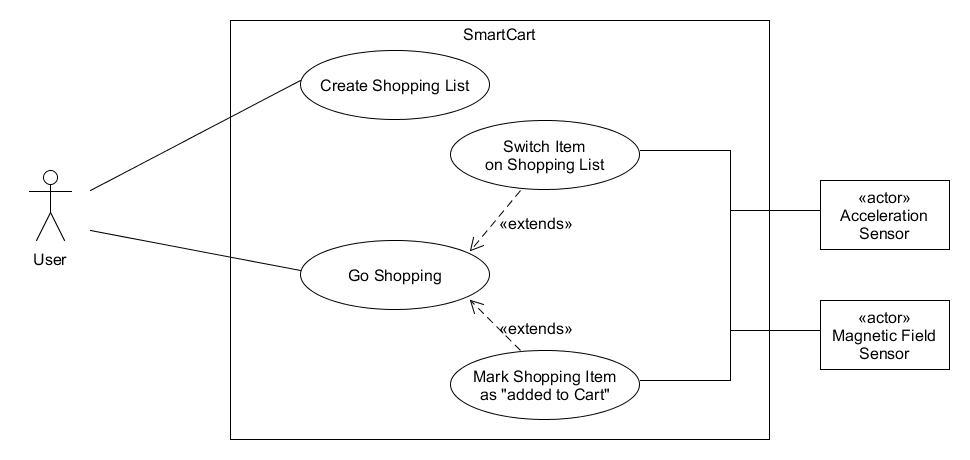
\includegraphics[width=\textwidth]{res/sa/useCaseDiagram.png}
\caption{Overview of the System's Use Cases}
\label{fig:UseCases}
\end{figure}

\subsection{Relations between the captured Gestures
and the used Sensors}

\label{sect:dataModel}
Figure \ref{fig:DataModel} shows a model of how the smartphone, the sensors and
the gestures that should be recognized are related to each other. The
acceleration sensor provides information about the smartphone's speed-up along
its coordinate axes. In the most cases, these axes are not aligned with the
standard x-y-z axes because of the smartphone's orientation. Since the
orientation affects the measured acceleration values, it has to be taken into
account when recognizing the user's gestures.

\begin{figure}
\centering
\captionsetup{justification=centering}
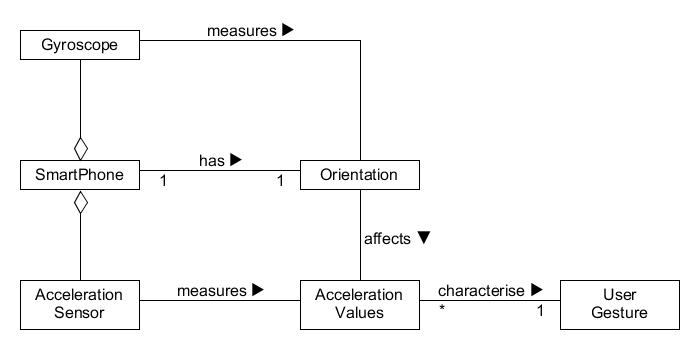
\includegraphics[width=\textwidth]{res/sa/UserGestureDataModel.png}
\caption{Data Model of the User Gestures to recognize}
\label{fig:DataModel}
\end{figure}

\subsection{Application Context}
The context of the application can be retrieved from figure \ref{fig:context}.
The inputs are the values of the accelerometer $a_x$, $a_y$ and $a_z$ as well as
the angles $azimuth$, $pitch$ and $roll$ that determine the smartphones
orientation. The current state and any other information of the application are
visualized on the smartphone's display.

\begin{figure}
\centering
\captionsetup{justification=centering}
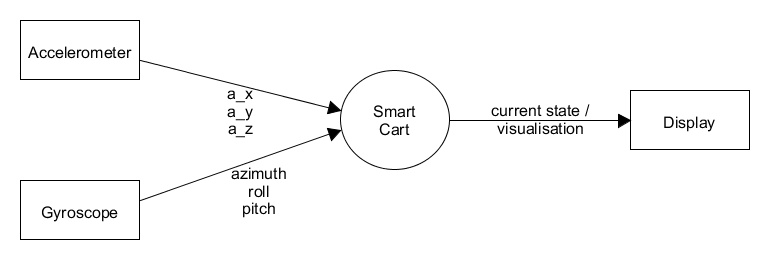
\includegraphics[width=\textwidth]{res/sa/ContextDiagram.png}
\caption{Context of the Application to develop}
\label{fig:context}
\end{figure}

\subsection{Finite State Machine}

The app SmartCart is developed as a finite state machine. A finite state machine
is defined by the fact that it can only have finite states. In order to describe
such a machine, the so-called state diagrams are used. The state diagrams
resulting from the analysis and evolved during the development cycle are
presented in the following subsections.

\subsubsection{First State Machine}

This section describes the first design of the state machine. As can be seen in
figure \ref{fig:first state machine}, this consists of only two states. The
reason for only two states is that at this early development cylce neither the
gestures nor the action triggered by the gestures could be accurately defined.
Therefore, a data analysis was first carried out to ensure which gestures are
possible at all and which make sense for the application.

\begin{figure}
\centering
\captionsetup{justification=centering}
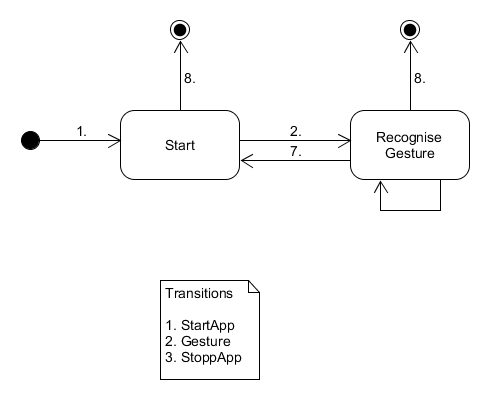
\includegraphics[width=\textwidth]{res/sa/PresentationStateMachineOld.png}
\caption{First Finite State Machine}
\label{fig:first state machine}
\end{figure}

\subsubsection{Evolution of the State Machine}

After the completion of the data analysis, the gestures and actions could be
defined (see section \ref{sec:bliblbablubb}) \textbf{\color{red}{TODO: Kapitle
vom Markus referenzieren}}. Subsequently, the state machine could also be
evolved and adapted. After starting the application, it is in the ``Start''
state. Afterwards, it is possible to start the purchase. If purchasing is
started with ``Start Shopping'', the application is in the ``Recognise
Gesture '' state. In this state, the application waits for a gesture. For this
purpose, two gestures were defined, each of lead to a certain action. If a
clockwise gesture of the mobile phone is detected, this leads to the state
``Check Item''. In this state, the selected item is checked off. Subsequently,
the state switches back to the ``Recognise Gesture'' state. If a
counter-clockwise gesture is detected, this results in the ``Switch Item''
state. In this state, the current item is swapped to the end of the shopping
list. After the action has been completed, the system returns to the previous
state. In general, the status `` Recognise Gesture '' will remain as long as no
valid gesture is detected or the purchase is terminated. In addition, it is
possible to terminate the app in all states. The complete state machine is shown
in figure \ref{fig:evo state machine}.

\begin{figure}
\centering
\captionsetup{justification=centering}
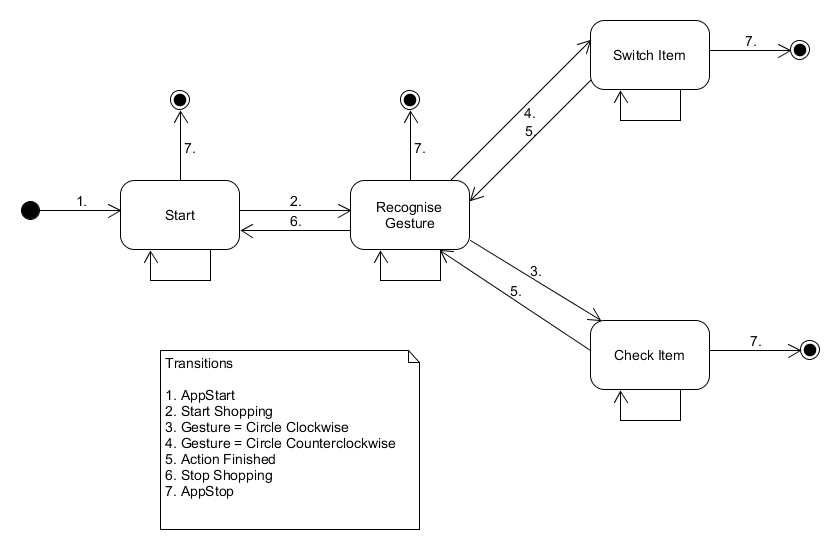
\includegraphics[width=\textwidth]{res/sa/PresentationStateMachineNew.png}
\caption{Evolutioned Finite State Machine}
\label{fig:evo state machine}
\end{figure}

